\documentclass[a4paper,10pt]{article}

% Encoding and typeface: XeLaTeX with Latin Modern Roman (fontspec default), English via polyglossia
\usepackage{fontspec}
\usepackage{polyglossia}
\setdefaultlanguage[variant=british]{english}

% Layout (tight margins)
\usepackage[a4paper,top=1.2cm,bottom=1.3cm,left=1.3cm,right=1.3cm]{geometry}

% Typography
\usepackage{microtype}
\usepackage{setspace}
\setstretch{0.92}

% Paragraph settings
\setlength{\parindent}{0pt}
\setlength{\parskip}{3pt}

% Section styling
\usepackage{titlesec}
\titleformat{\section}{\bfseries\normalsize}{\thesection.}{0.4em}{}
\titlespacing*{\section}{0pt}{6pt}{3pt}

% Better lists
\usepackage{enumitem}
\setlist{noitemsep, topsep=2pt}

% Mathematics, tables, figures
\usepackage{amsmath}
\usepackage{booktabs}
\usepackage{graphicx}
\usepackage[font=small,labelfont=bf,labelsep=period,skip=3pt]{caption}
\setlength{\textfloatsep}{8pt}
\setlength{\floatsep}{6pt}

\newcommand{\ExOnePeriod}{56{,}826}
\newcommand{\ExOneShare}{0.72}
\newcommand{\ExTwoTail}{2}
\newcommand{\ExTwoPeriod}{14{,}076}
\newcommand{\ExTwoShare}{0.14}
\newcommand{\ExTwoGcd}{3}
\newcommand{\ExThreePeriod}{8}
\newcommand{\VOneStepTwo}{14{,}079}
\newcommand{\ReadmeStated}{27, 9, 3, 1, 11, 23, 29}
\newcommand{\ReadmeComputed}{27, 9, 3, 1, 11, 25, 19, 17, 27}
\newcommand{\NuOne}{1079.0}
\newcommand{\NuOneNorm}{0.357}
\newcommand{\NuOneSpacing}{0.00093}
\newcommand{\NuTwo}{1722.0}
\newcommand{\NuTwoNorm}{0.508}
\newcommand{\NuTwoSpacing}{0.00058}
\newcommand{\BatteryN}{10{,}000}
\newcommand{\BatteryTests}{36}
\newcommand{\BatteryExpectedFalse}{0.36}
\newcommand{\BatteryRejections}{0}
\newcommand{\BatteryMinP}{0.029}
\newcommand{\BatteryMinPGen}{Mersenne-Twister (R)}
\newcommand{\SerialN}{300{,}000}
\newcommand{\RanduChi}{80{,}064}
\newcommand{\SerialDf}{7{,}999}
\newcommand{\RanduTriples}{299{,}998}
\newcommand{\RanduPlanes}{15}
\newcommand{\RanduPlaneMin}{-5}
\newcommand{\RanduPlaneMax}{9}
\newcommand{\PerfCycleSize}{32{,}768}
\newcommand{\PerfCycleVOne}{2.14}
\newcommand{\PerfCycleVTwo}{0.018}
\newcommand{\PerfCycleRatio}{120}
\newcommand{\PerfCycleMax}{16{,}777{,}216}
\newcommand{\PerfCycleMaxTime}{8.9}
\newcommand{\PerfGenVOne}{0.69}
\newcommand{\PerfGenVTwo}{0.16}
\newcommand{\PerfGenRatio}{4.3}
\newcommand{\PerfMachine}{R 4.5.1}
\newcommand{\SlopeVOne}{2.03}
\newcommand{\SlopeVTwo}{0.99}


\begin{document}

% Header (top-right)
\begin{flushright}
\small \textbf{Compiled on:} \today
\end{flushright}

\vspace{-6pt}
\hrule
\vspace{24pt}

\textbf{TITLE:} Linear congruential generator (LCG): period, lattice structure and empirical tests

\textbf{SUBJECT:} Aim, method and results of the analyses in version 2 of the \texttt{linear-congruential-generator} repository

\textbf{PREPARED BY:} Muhammed İkbal Yılmaz (myucanlar@gmail.com)

\vspace{12pt}

\section{Aim and scope}

Starting from a seed $x_0$, the linear congruential generator (LCG) produces the sequence
\[
  x_{n+1} = (a\,x_n + c) \bmod m, \qquad u_n = x_n/m \in [0,1),
\]
where $a$ is the multiplier, $c$ the increment and $m$ the modulus. The sequence is fully deterministic, so whether a
generator is good comes down to two questions: \emph{how many numbers can it produce} (the period) and \emph{how independent
do successive numbers look} (the lattice structure and the tests). This note contains four analyses, each answering one of
these questions:

\begin{enumerate}
  \item \textbf{Period:} How many numbers does the generator give before it repeats itself?
  \item \textbf{Lattice structure:} How are successive pairs of numbers spread over the unit square?
  \item \textbf{Empirical tests:} Can classical tests detect the weaknesses seen in analyses 1 and 2?
  \item \textbf{Running time:} Does the new code really remove the limits of version 1?
\end{enumerate}

The six generators were chosen deliberately: the three examples of version 1 (the main object of study) and three reference
points from the literature. \textbf{RANDU} ($a=65539$, $c=0$, $m=2^{31}$) is a generator with a well-known defect and is used to
check whether the tests can find it. \textbf{MINSTD} ($a=16807$, $c=0$, $m=2^{31}-1$) is the multiplicative generator with the
longest possible period proposed by Park and Miller (1988). The \textbf{rand48 parameters} ($a=25{,}214{,}903{,}917$, $c=11$,
$m=2^{48}$) represent the case in which the product exceeds R's numerical precision. The \textbf{Mersenne-Twister}, which is
not an LCG (R's default generator; Matsumoto and Nishimura, 1998), was used as the benchmark in the tests.

\section{Method}

The code uses base R only. Every result was checked in the unit tests against an independent computation: a brute-force
search, a plain loop, or reference values computed with exact integer arithmetic.

\begin{itemize}
  \item \textbf{Exact arithmetic.} R stores numbers in double precision, which represents every integer up to $2^{53}$
  exactly. Once $a\,x_n$ exceeds that limit, the result is silently wrong. With the rand48 parameters, direct computation
  departs from the exact sequence at the second value. The code therefore splits $a$ into digits in base $2^s$ and computes
  $a x \bmod m$ by Horner's rule, so that no intermediate value reaches $2^{53}$. The method is exact for $m \le 2^{51}$.
  \item \textbf{Jumping ahead.} After $k$ steps the map is still affine: $x_{n+k} = (A_k x_n + C_k) \bmod m$. $(A_k, C_k)$ is
  found by binary exponentiation in $O(\log k)$ steps (Brown, 1994). Numbers are generated in blocks of length $\sqrt{n}$;
  each block follows from the previous one by a single vector operation.
  \item \textbf{Tail and cycle.} In a finite state space every sequence first passes through a tail of length $\mu$ and then
  enters a cycle of length $\lambda$. Brent's (1980) algorithm finds $\lambda$ with constant memory, and $\mu$ follows from a
  jump ahead. Version 1 compared every new value with all earlier ones; this takes $O((\mu+\lambda)^2)$ operations and gives
  only $\mu+\lambda$.
\end{itemize}

\section{Analysis 1: Period (Table~\ref{tab:period})}

\textbf{Why.} The period is the largest number of values that can be taken from a generator. A sample longer than the period
repeats the same numbers in the same order, and simulation results are then not based on independent observations. The period
is not estimated from a sample; it is computed exactly from the theory.

\textbf{Method.} For $c \ne 0$ the Hull--Dobell theorem applies. By the theorem, the period equals $m$ for every seed if and
only if three conditions hold: (i) $c$ and $m$ are coprime, (ii) $a-1$ is divisible by every prime factor of $m$, (iii) if 4
divides $m$, then 4 divides $a-1$ (Hull and Dobell, 1962). The theorem does not cover the case $c=0$. There, for a seed coprime
to $m$, the period is the multiplicative order of $a$ modulo $m$; this order is at most the Carmichael function $\lambda(m)$
(Knuth, 1997, §3.2.1.2). Where the theory does not give the answer directly, Brent's algorithm was used.

\begin{table}[h]
\centering\footnotesize\setlength{\tabcolsep}{4pt}
\caption{Hull--Dobell conditions and tail and cycle lengths (seed $x_0=1$; $x_0=27$ for example 3). The conditions are shown
only for $c\ne0$.}\label{tab:period}
\begin{tabular}{lrrlccccrl}
\toprule
 & & & & \multicolumn{3}{c}{Hull--Dobell} & & & \\
\cmidrule(lr){5-7}
Generator & $a$ & $c$ & $m$ & (i) & (ii) & (iii) & Tail & Cycle & Method \\
\midrule
Version 1, example 1 & 1{,}079 & 863 & $7\cdot 11\cdot 19\cdot 5413$ & yes & no & yes & 0 & 56{,}826 & Brent \\
Version 1, example 2 & 1{,}722 & 990 & $3^{2}\cdot 13\cdot 139\cdot 613$ & no & no & yes & 2 & 14{,}076 & Brent \\
Version 1, example 3 & 11 & 0 & $2^{5}$ & -- & -- & -- & 0 & 8 & order of $a$ \\
RANDU & 65{,}539 & 0 & $2^{31}$ & -- & -- & -- & 0 & $2^{29}$ & order of $a$ \\
MINSTD (Park--Miller) & 16{,}807 & 0 & $2^{31}-1$ & -- & -- & -- & 0 & $2^{31}-2$ & order of $a$ \\
rand48 parameters & 25{,}214{,}903{,}917 & 11 & $2^{48}$ & yes & yes & yes & 0 & $2^{48}$ & Hull--Dobell \\
\bottomrule

\end{tabular}
\end{table}

\textbf{Finding and interpretation.} The cycles of the two large examples of version 1 contain only \ExOnePeriod{} and
\ExTwoPeriod{} numbers, which is \ExOneShare\% and \ExTwoShare\% of their moduli. Example 1 fails condition (ii):
$a-1 = 1078 = 2\cdot7^2\cdot11$ is not divisible by 19 or 5413, which are factors of $m$. Example 2 fails (i) and (ii). In
addition, $a$ and $m$ have the common divisor \ExTwoGcd{}, so the map is not one-to-one, and the sequence passes through a tail
of \ExTwoTail{} values before it enters the cycle. Version 1 reported \VOneStepTwo{} for this example; that number does not
separate the tail from the cycle. Example 3 is multiplicative ($c=0$); its period of \ExThreePeriod{}, that is $\lambda(32)$, is
the largest value attainable. The version 1 README gave the sequence \ReadmeStated{} for this example; the correct sequence is
\ReadmeComputed. In practice, any simulation that uses more than a few thousand numbers from these two generators reuses the
same numbers.

\section{Analysis 2: Lattice structure (Figure~\ref{fig:lattice})}

\textbf{Why.} A long period is not enough by itself. In an LCG, $u_{n+1}$ is a linear function of $u_n$ (mod 1). The pairs
$(u_n, u_{n+1})$ therefore fall on parallel lines in the unit square. The larger the gap between the lines, the larger the
regions of the square that are never visited.

\textbf{Method.} The spectral test (Knuth, 1997, §3.3.4) measures this gap with a single number. $\nu_2$ is the length of the
shortest non-zero vector $(s_1,s_2)$ with $s_1 + a s_2 \equiv 0 \pmod m$, and the largest distance between adjacent lines is
$1/\nu_2$. Since $\nu_2 \le (4/3)^{1/4}\sqrt{m}$, its ratio to this upper bound is a scale-free measure between 0 and 1; values
close to 1 are good (L'Ecuyer, 1999). The vector $(-a, 1)$ always satisfies the condition, so $\nu_2 \le \sqrt{a^2+1}$: a small
multiplier means lines that are far apart. The shortest vector was found by Lagrange--Gauss reduction; the method is exact for
$m \le 2^{26}$.

\textbf{Why the figure is drawn this way.} $\nu_2$ is a single number; the figure shows what it means. The lines are about
0.001 apart, so they cannot be seen on the whole unit square. The figure therefore shows the pairs with $u_n < 0.004$ out of one
full period of example 1 (\ExOnePeriod{} pairs). For comparison, the same number of Mersenne-Twister pairs is shown in the
second panel. Without a lattice structure the points scatter.

\begin{figure}[h]
\centering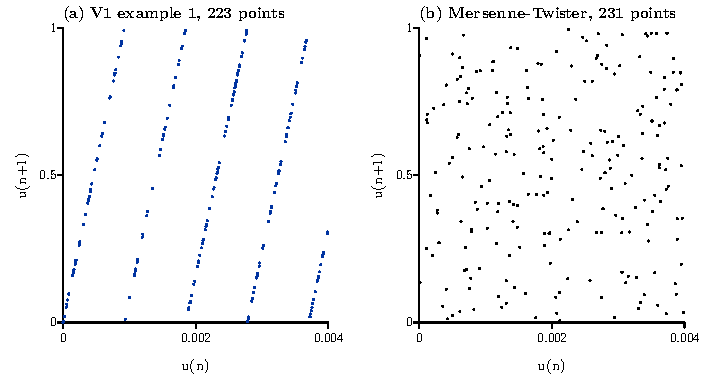
\includegraphics[width=0.86\linewidth]{../figures/fig1_pairs.pdf}
\caption{Successive pairs $(u_n, u_{n+1})$ with $u_n < 0.004$. Left: example 1 of version 1, full period. Right: the same
number of Mersenne-Twister pairs.}\label{fig:lattice}
\end{figure}

\textbf{Finding and interpretation.} For example 1, $\nu_2 = \NuOne$, the distance between lines is $\NuOneSpacing$ and the
normalised value is $\NuOneNorm$. For example 2 these values are $\NuTwo$, $\NuTwoSpacing$ and $\NuTwoNorm$. In the figure,
the points in the left panel gather on a few lines of slope $a$, while the right panel shows no pattern. A normalised value far
from 1 shows that the multiplier was poorly chosen with respect to the lattice structure.

\section{Analysis 3: Empirical tests (Table~\ref{tab:tests}, Figure~\ref{fig:randu})}

\textbf{Why.} In practice, generators are mostly assessed with statistical tests. This analysis tests the power of the tests:
can classical tests reveal a defect that is known from theory (the examples of version 1, RANDU)?

\textbf{Method.} \BatteryN{} numbers were taken from each generator and six classical tests were applied (Knuth, 1997,
§3.3.2): equidistribution on 100 cells ($\chi^2$), Kolmogorov--Smirnov, serial tests on non-overlapping pairs and triples, lag-1
autocorrelation, and the runs-up-and-down test. Non-overlapping groups were used so that the cell counts are multinomial and
the $\chi^2$ reference distribution is valid. The significance level is 0.01. Over \BatteryTests{} tests, about
\BatteryExpectedFalse{} false rejections are expected even if all generators were flawless. A serial test of triples on a
finer grid ($20^3$ cells) was then run on \SerialN{} numbers.

\begin{table}[h]
\centering\footnotesize\setlength{\tabcolsep}{4pt}
\caption{$p$-values. First six columns: \BatteryN{} numbers per generator. Last column: non-overlapping triples, $20^3$
cells, \SerialN{} numbers.}\label{tab:tests}
\begin{tabular}{lccccccc}
\toprule
 & Equidistribution & KS & Pairs & Triples & Autocorrelation & Runs & Triples, $20^3$ \\
\midrule
Version 1, example 1 & 0.843 & 0.707 & 0.069 & 0.477 & 0.332 & 0.033 & period too short \\
Version 1, example 2 & 0.645 & 0.711 & 0.832 & 0.215 & 0.405 & 0.806 & period too short \\
RANDU & 0.387 & 0.814 & 0.578 & 0.661 & 0.184 & 0.351 & $<$0.001 \\
MINSTD (Park--Miller) & 0.554 & 0.695 & 0.946 & 0.536 & 0.960 & 0.181 & 0.605 \\
rand48 parameters & 0.643 & 0.935 & 0.188 & 0.676 & 0.549 & 0.874 & 0.593 \\
Mersenne-Twister (R) & 0.029 & 0.389 & 0.688 & 0.965 & 0.843 & 0.312 & 0.994 \\
\bottomrule

\end{tabular}
\end{table}

\textbf{Finding.} None of the \BatteryTests{} tests rejected at the 0.01 level; the smallest $p$-value (\BatteryMinP{})
belongs to the \BatteryMinPGen{}, which serves as the benchmark. Classical tests on small samples did not reveal the weaknesses
of analyses 1 and 2. In the fine-grid test of triples, RANDU was clearly rejected ($\chi^2 = \RanduChi$ on \SerialDf{} degrees
of freedom). The two examples of version 1 could not even take this test, because a sample of \SerialN{} numbers would repeat
their cycle several times.

\textbf{Why the figure is drawn.} The test says that RANDU's triples are not uniformly distributed, but not why. The reason is
algebraic: since $a = 2^{16}+3$, $a^2 = 2^{32} + 6\cdot2^{16} + 9 \equiv 6a - 9 \pmod{2^{31}}$, and therefore
$9u_k - 6u_{k+1} + u_{k+2}$ is an integer for every $k$. The figure shows the distribution of this combination. For RANDU, all
\RanduTriples{} triples gather on the \RanduPlanes{} integers from $\RanduPlaneMin$ to $\RanduPlaneMax$; that is, every triple
lies on one of \RanduPlanes{} parallel planes in the unit cube (Marsaglia, 1968). For MINSTD, which has a modulus of the same
size, the values spread continuously.

\begin{figure}[h]
\centering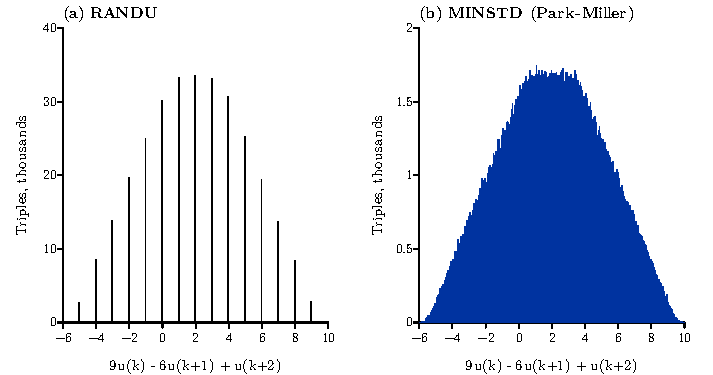
\includegraphics[width=0.86\linewidth]{../figures/fig2_randu_planes.pdf}
\caption{Histogram of $9u_k - 6u_{k+1} + u_{k+2}$ over \RanduTriples{} consecutive triples (bin width 0.05).}\label{fig:randu}
\end{figure}

\textbf{Interpretation.} Passing a few tests is a necessary condition for a generator, not a sufficient one. Serious
assessments use large test batteries such as TestU01 (L'Ecuyer and Simard, 2007). The period and the lattice structure of an LCG,
by contrast, can be computed exactly from the theory without being estimated by tests.

\section{Analysis 4: Running time (Figure~\ref{fig:time})}

\textbf{Why.} The repetition check of version 1 had a cost that grows with the square of the cycle length. In practice this
limited the periods that could be analysed. This analysis measures how large the improvement is and where it comes from.

\textbf{Method.} Generators $x \mapsto (5x+1) \bmod 2^k$ satisfy the Hull--Dobell conditions, so their cycle length is exactly
$2^k$; this keeps the problem size under control. Each time is the median of three measurements. So that short calls do not
fall below the resolution of the timer, each measurement was repeated until it lasted at least 0.2 seconds.

\textbf{How to read the figure.} The axes are logarithmic. A time that grows as $n^k$ appears on these axes as a straight line
of slope $k$, so the order of growth can be read directly. The least-squares slope is \SlopeVOne{} for version 1 (quadratic)
and \SlopeVTwo{} for version 2 (linear).

\begin{figure}[h]
\centering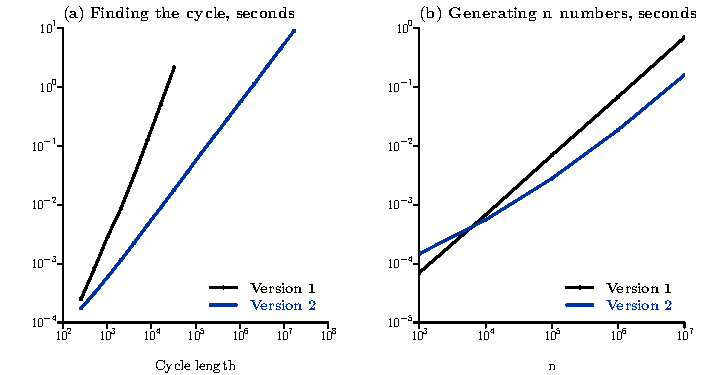
\includegraphics[width=0.86\linewidth]{../figures/fig3_performance.pdf}
\caption{Running time, median of three measurements (\PerfMachine). Left: finding the cycle (version 1 only up to $2^{15}$).
Right: generating $n$ MINSTD numbers.}\label{fig:time}
\end{figure}

\textbf{Finding.} Version 1 finds a cycle of length \PerfCycleSize{} in \PerfCycleVOne{} seconds, version 2 in
\PerfCycleVTwo{} seconds (about \PerfCycleRatio{} times faster). Version 2 finds a cycle of length \PerfCycleMax{} in
\PerfCycleMaxTime{} seconds. For number generation both methods are linear and differ by a constant factor: $10^7$ numbers take
\PerfGenVOne{} seconds with a plain loop and \PerfGenVTwo{} seconds with blocked jumps (a factor of \PerfGenRatio). For a few
thousand numbers the plain loop is faster. Absolute times depend on the machine; the order of growth does not.

\section{Conclusions and limitations}

\begin{itemize}
  \item The parameters of version 1 were not chosen by any criterion. The Hull--Dobell conditions, the multiplicative order and
  the spectral test show their weaknesses directly. Classical tests on samples shorter than the period do not.
  \item Moduli above $2^{51}$ (e.g.\ the $2^{64}$ used by many current LCGs) require big-integer arithmetic and are not
  supported. The spectral test is two-dimensional and is computed for $m \le 2^{26}$.
  \item The test battery is small; its purpose is to illustrate, not to certify a generator. Times were measured on a single
  machine.
  \item LCGs are not suitable for cryptographic purposes. For simulation, R's built-in generators should be preferred.
\end{itemize}

\section*{References}
{\small
Brent, R. P. (1980). An improved Monte Carlo factorization algorithm. \textit{BIT}, 20, 176--184.\\
Brown, F. B. (1994). Random number generation with arbitrary strides. \textit{Trans.\ American Nuclear Society}, 71, 202--203.\\
Hull, T. E. and Dobell, A. R. (1962). Random number generators. \textit{SIAM Review}, 4(3), 230--254.\\
Knuth, D. E. (1997). \textit{The Art of Computer Programming, Vol.\ 2: Seminumerical Algorithms}, 3rd ed. Addison-Wesley.\\
L'Ecuyer, P. (1999). Tables of linear congruential generators of different sizes and good lattice structure.
\textit{Mathematics of Computation}, 68, 249--260.\\
L'Ecuyer, P. and Simard, R. (2007). TestU01: A C library for empirical testing of random number generators.
\textit{ACM Trans.\ Mathematical Software}, 33, Article 22.\\
Marsaglia, G. (1968). Random numbers fall mainly in the planes. \textit{PNAS}, 61(1), 25--28.\\
Matsumoto, M. and Nishimura, T. (1998). Mersenne Twister: A 623-dimensionally equidistributed uniform pseudo-random number
generator. \textit{ACM Trans.\ Modeling and Computer Simulation}, 8(1), 3--30.\\
Park, S. K. and Miller, K. W. (1988). Random number generators: Good ones are hard to find. \textit{Communications of the ACM},
31(10), 1192--1201.

\smallskip
An AI coding assistant was used in writing the code and in preparing this note. All numbers are generated from
\texttt{figures/*.csv} by \texttt{make\_paper.R}.
}

\end{document}
